\subsubsection{General Introduction to Photon Detection}
\label{introReceiver}
Photon detection typically occurs in a two-step process: the absorbed photon creates a measurable change in the detector's electrical properties, and the changes is registered in an external read-out integrated circuit (\acs{ROIC}). In general, the detector material responds either \textit{directly} to the incident photon by generating a free charge, with this charge then being responsible for producing the change in electrical properties, or \textit{indirectly}, with the absorbed optical power generating a temperature rise in the detector material, which is responsible for producing the change in electrical properties. In either case, this photon-induced analog signal is registered and amplified in the \acs{ROIC} digitization for further signal processing. 

Additional factors include the detector material \textit{sensitivity} and the detector \textit{device speed of response}. Sensitivity is a measure of how few photons are required to raise the detector output above any background noise level present in the absence of incident light. Response speed is a measure of how faithfully the detector's electrical output responds to changes in the intensity of the input light signal.

\subsubsubsection{Solide-State Photon Detection}
\label{ssphotonsensing}
Solid-state imaging is based on the physical principle of converting light (photons) into a measurable quantity (electrical voltage, electrical current). Photons falling onto and penetrating into a semiconductor substrate can transfer part of their energy to the substrate by generating electron-hole pairs. For an n-type semiconductor, if the energy content of the photons is high enough, electrons can be released from the valence band and swept into the conduction band, leaving behind a hole in the valence band. To generate an electron-hole pair, the energy of the photons has to be larger than the bandgap of the semicondector substrate.

For reasons of cost and miniaturization, a solid state solution for single photon detection is highly desirable. Figure \ref{fig:intro_receiver1} on page \ref{fig:intro_receiver1} shows a classification that covers the current state-of-the-art on optical solid-state 3D image sensors. 

\begin{figure}
\centering
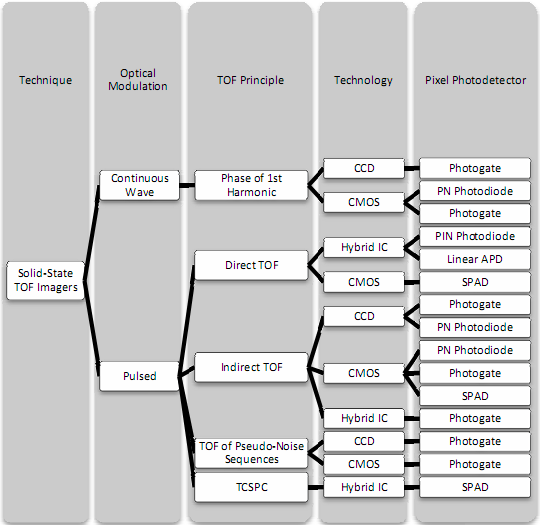
\includegraphics[scale = 1]{chapters/img/intro_receiver1.png}
\caption{Classification of state-of-the-art optical TOF image sensors.}
\label{fig:intro_receiver1}
\end{figure}

